%  This is a LaTex file.

%  Homework for the course "AMath 585:  Applied Linear Algebra and Numerical Analysis",
%  Autumn quarter, 2009, Anne Greenbaum.


%   A latex format for making homework assignments.


\documentclass[letterpaper,12pt]{article}

%          The page format, somewhat wider and taller page than in art12.sty.

\topmargin -0.1in \headsep 0in \textheight 8.9in \footskip 0.6in
\oddsidemargin 0in  \evensidemargin 0in  \textwidth 6.5in
\usepackage{graphicx}
\usepackage{listings}
\usepackage{caption}
\usepackage{subcaption}
\usepackage{color}
\usepackage{float}
\usepackage{tikz}
\definecolor{keywords}{RGB}{255,0,90}
\definecolor{comments}{RGB}{0,0,113}
\definecolor{red}{RGB}{160,0,0}
\definecolor{green}{RGB}{0,150,0}
\definecolor{codegreen}{rgb}{0,0.6,0}
\definecolor{codegray}{rgb}{0.5,0.5,0.5}
\definecolor{codepurple}{rgb}{0.58,0,0.82}
\definecolor{backcolour}{rgb}{0.95,0.95,0.92}
\definecolor{brown}{rgb}{0.59, 0.29, 0.0}
\definecolor{beaublue}{rgb}{0.74, 0.83, 0.9}
\definecolor{orange}{rgb}{1.0, 0.5, 0.0}
\definecolor{darkslategray}{rgb}{0.18, 0.31, 0.31}
\definecolor{deepblue}{rgb}{0,0,0.5}
\definecolor{deepred}{rgb}{0.6,0,0}
\definecolor{deepgreen}{rgb}{0,0.5,0}
\lstdefinestyle{myMatlabstyle}{
	language=Matlab,
	backgroundcolor=\color{white},
	commentstyle=\color{codegreen},
	keywordstyle=\color{blue},
	%identifierstyle=\color{brown},
	numberstyle=\tiny\color{codegray},
	stringstyle=\color{orange},
	basicstyle=\footnotesize,
	breakatwhitespace=false,
	breaklines=true,
	captionpos=b,
	keepspaces=true,
	numbers=left,
	numbersep=5pt,
	showspaces=false,
	showstringspaces=false,
	showtabs=false,
	tabsize=2
}
\lstdefinestyle{myPythonstyle}{
	language=Python,
	basicstyle=\ttfamily\small,
	keywordstyle=\color{blue},
	backgroundcolor=\color{white},
	commentstyle=\color{green},
	stringstyle=\color{red},
	showstringspaces=false,
	%identifierstyle=\color{brown},
	breaklines=true,
}
\lstset{language=Matlab,frame=single}
\lstset{language=Python,frame=single}
\usepackage{amsmath}
\usetikzlibrary{decorations.pathreplacing}
\usepackage{epsfig}         % to insert PostScript figures
       % to insert PostScript figures

\begin{document}


%          Definitions of commonly used symbols.



%          The title and header.

\noindent
{\scriptsize ES$\_$APPM 420-1, Fall 2018} \hfill

\begin{center}
\large
Assignment 1.
\normalsize

Jithin D. George
\end{center}

\noindent
Due Oct 9
\vspace{.3in}

%           The questions!



\noindent


\begin{enumerate}
\item
\begin{enumerate}
\item
From the conservation of mass, the total mass of water in the pipe should be conserved, i.e

\[\frac{d}{dt}\int_{container} (\rho V)=0\]
where $\rho$ is density and V is Volume. In incompressible flow, density is constant.

\[\rho \frac{d}{dt}\int_{container} ( V)=\rho \int_{container} \frac{dV}{dt} = \rho \int_{0}^h A(h ) v(h) =0\]
where v(h) is the velocity at height h.
Thus,
\[A(h)v(h)=A(0)v(0)\]
\[v(h)=\frac{A(0)v(0)}{A(h)} = - 0.6 \sqrt{2gh}\frac{A(0)}{A(h)}\]
\item
 \[\frac{dh}{dt}= -0.6 A(0)\frac{\sqrt{2gh}}{A(h)}\]

  \[h^{c-0.5} dh = -0.6 A(0)\sqrt{2g} dt\]
	  \[\frac{h^{c+0.5}}{c+0.5}  = -0.6 A(0)\sqrt{2g} t+\frac{h_0^{c+0.5}}{c+0.5}\]
			  \[h^{c+0.5}  = -0.6 A(0)(c+0.5)\sqrt{2g} t+h_0^{c+0.5}\]
However, we would have $A(0)= 0^C$. So,
 \[h^{c+0.5}  = h_0^{c+0.5}\]
  \[h  = h_0\]
	Thus, according to this model, the height stays the same. This is not physical when there is an outflow of water (violates conservation of mass).
\end{enumerate}

\item
\begin{enumerate}
\item
Using grams for Mass and minutes for time, we get
\[ M = 5 -5 e^{-t}\]
If $y$ is the mass in kg and $\tau$ is the time in minutes,
\[ y = \frac{M}{1000}, \tau = \frac{t}{60}\]
So, we have
\[ 1000 y = 5 -5 e^{-60\tau }\]
\[ y = \frac{5}{1000} -\frac{5}{1000} e^{-60\tau }\]
\item
We start with
\[ M = 5 -5 e^{-t}\]
where everything is a particular system, say SI. So, if we have $C_1 = 1 kg^{-1}, C_2 = 1 s^{-1}$.

Thus, we still have
\[ C_1 M = 5 -5 e^{-C_2 t}\]

Suppose we change to another set of units. Then,
\[M = \alpha M' , t = \beta t'\]
But we also will have
\[C_1 = \frac{1}{\alpha} C_1' , C_2 = \frac{1}{\beta} C_2'\]

Thus, we'll end up with
\[ C_1' M' = 5 -5 e^{-C_2' t'}\]
which is the same complete equation.
\end{enumerate}

\item

\textbf{Using dimensional analysis}

We know that the height $h : [L]$ depends on the pressure $P: [ML^{-1}T^{-2}]$, density of the oil $\rho : [ML^{-3}]$ and acceleration due to gravity $g: [LT^{-2}]$. There are 3 variables and 4 dimensions. So, from Buckingham Pi, there must be one dimensionless parameter $\pi$.



Equating  height to an arbitary formula of the other terms, we have

\[\pi  = h^-1P^ag^b\rho^cA^d\]
\[1 = L^{-1}M^aL^{-a}T^{-2a}L^bT^{-2b}M^cL^{-3c}\]
\[1 = M^{a+c}L^{b-a-3c-1}T^{-2a-2b}\]

\begin{align*}
a+c&=0\\
b-a-3c-1&=0\\
-2a-2b &=0
\end{align*}
 we get a =1, b = -1 and c = -1. That implies
\[\pi  = \frac{P}{\rho g h}\]
We know for some function $f$,
\[f(\pi)=0\]
This function would have some root $c$. Thus,
\[\pi = c\]
\[\frac{P}{\rho g h}= c\]
\[h  = c \frac{P}{\rho g }\]
Using a data point, we can find that c = 1.


\textbf{Using force balance on a column of water }

\begin{tikzpicture}
\draw [draw=black] (3,4.5) rectangle (4,1.3);
\draw [decorate,decoration={brace,amplitude=10pt},xshift=-4pt,yshift=0pt]
(2.5,1.5) -- (2.5,4.5) node [black,midway,xshift=-0.6cm]
{\footnotesize $h$};

\draw[->](3.5,1.6) -- (3.5,1)  ;

\draw[->](3.5,-0.7) -- (3.5,0) ;
\node at (3.5,0.7) {$mg$};
\node at (3.5,-1) {$PA$};
\end{tikzpicture}

Fromthe force balance, we have
\[PA = mg\]
\[PA = \rho V g\]
\[PA = \rho A h g\]
\[h = \frac{P}{\rho g}\]
\item

\begin{enumerate}
\item
Here, position is positive downwards in the direction of gravity.
\[x'' = g+k|x'|^2\]
Note that $k$ is not the spring constant , but the spring constant divided by mass.
\item
\[v' = g+k|v|^2\]
\item
 The solution to the above ode is
 \[v = \sqrt{\frac{g}{k}} \tan(c_1 \sqrt{gk}+  \sqrt{gk}t)\]
 Since our initial velocity is 0,
  \[v = \sqrt{\frac{g}{k}} \tan(  \sqrt{gk}t)\]
	Thus, the position is given by
	\[x = \frac{1}{k} \log(|\sec(\sqrt{gk}t)|) \]

	This blows up when $\sqrt{gk}t = \frac{\pi}{2}$. In the plots, we see that it is point of divergence. So,
	\[t_c = \frac{\pi}{2\sqrt{gk}}\]

\item
 Plots
\begin{figure}[H]
\begin{centering}
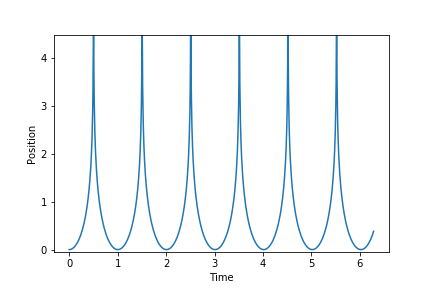
\includegraphics[width=4in]{Position.png}
\caption{Position versus time}
\end{centering}
\end{figure}


\begin{figure}[H]
\begin{centering}
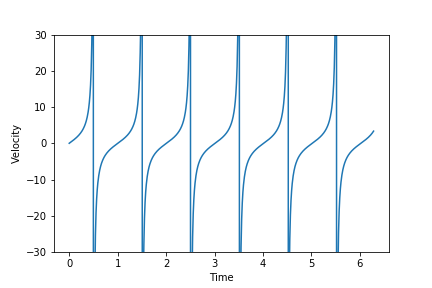
\includegraphics[width=4in]{Velocity.png}
\caption{Velocity versus time}
\end{centering}
\end{figure}

Of course, the analytical solution is only valid as a model until $t_c = \frac{\pi}{2\sqrt{gk}}$. It doesn't make any physical sense for a ball to go to infinity and return without the presence of any attractive force.
\item

In that case, the position would be given by
\[x(t)= \frac{g}{k^2}e^{kt}-\frac{g}{k}\]
This does not blow up anywhere and hence there is no time of divergence.
This is a bad model because you should expect things to go very far away in finite time if drag and gravity acted in the same direction.

\end{enumerate}


\item
 Let the distance between the centers of the dice be $x$. Thus, the dynamics of the dice are given by
 \begin{align*}
x_1'' = \frac{Gm}{x^2}\\
x_2'' = -\frac{Gm}{x^2}\end{align*}

\[x'' = (x_2-x_1)'' = -\frac{2Gm}{x^2}\]
\[2x'x''  = -\frac{4Gmx'}{x^2}\]
\[(x')^2  = C+\frac{4Gm}{x}\]
Since the initial velocity is zero,
\[ C=- \frac{4Gm}{10^{-1}}\]
All units are SI to match with the G.
\[ x' = - \sqrt{- \frac{4Gm}{10^{-2}}+\frac{4Gm}{x}}=- 2\sqrt{Gm}\sqrt{- 10+\frac{1}{x}}\]
Here, the negative square root is taken because gravity is an attactive force and velocity is in the opposite direction of displacement.

Total time till collision is given by
\begin{align*}
T &= \int_{0.1}^0 dt\\
&= \int_{0.1}^0 \frac{dx}{v}\\
&= - \frac{1}{2\sqrt{Gm}} \int_{0.1}^0 \frac{dx}{\sqrt{- 10+\frac{1}{x}}}\\
&\approx - \frac{1}{2\sqrt{Gm}} \int_{0.1}^{0.001} \frac{dx}{\sqrt{- 10+\frac{1}{x}}}\\
&\approx \frac{0.0497}{2\sqrt{Gm}} \\
&\approx 9621 s
\end{align*}
\item
\begin{enumerate}
\item

Assume $l_1 > l_2$. The push of the first spring should balance the pull of the second spring so as to have equilibrium. Thus, the equilibrium position $x_0$ is in between the $l_1$ and $l_2$.

\[ k_1(l_1-x_0)=k_2(x_0-l_2)\]
\[x_0 = \frac{k_1 l_1 + k_2 l_2}{k_1 + k_2} \]

\item
If the mass is given a small perturbation $\Delta x$ about $x_0$, the position of the mass would be given by
\[x = x_0 + \Delta x\]
Its motion can be estimated from the forces acting on it.
\[mx'' =k_1(l_1-x) -k_2(x-l_2)\]
\[mx'' = -k_1(x-l_1) -k_2(x-l_2)\]
\begin{align*}
mx''  = -k_1(x-l_1) -k_2(x-l_2) \\
 = -(k_1+k_2)x +k_1 l_1 + k_2 l_2\\
\end{align*}

Writing the position as relative to the equilibrium,
\begin{align*}
m(x_0+\Delta x)''
 &= -(k_1+k_2)(x_0+\Delta x) +k_1 l_1 + k_2 l_2\\
 &= -(k_1+k_2)\Delta x
\end{align*}

\[\Delta x'' = -\frac{k_1+k_2}{m}\Delta x\]

Thus, the mass follows an S.H.M about $x_0$ .

\item

The solution to $y'' = -\frac{k_1+k_2}{m}y$ is $c_1 \sin(\sqrt{\frac{k_1+k_2}{m}}t)+ c_2 \cos(\sqrt{\frac{k_1+k_2}{m}}t)$. So, the period of oscillation is $\frac{2 \pi\sqrt{m}}{\sqrt{k_1+k_2}}$

\item

Since the dynamics are governed by
\[\Delta x'' = -\frac{k_1+k_2}{m}\Delta x\]
which can be written as
\[ x'' = -\frac{k_1+k_2}{m}(x-x_0)\]
we can see that a system equivalent to this must have the spring constant $\frac{k_1+k_2}{m}$ and an unstretched length $x_0$.


\end{enumerate}
\item
For the spings to be at rest, the spring should be at their unstretched lengths. The massless point with be at $l_1$ and the mass would be at $l_1 + l_2$ which would the equilibrium positions.


Let $x_2$ and $x_1$ be the perturbations about the equilibrium positions of the mass and the unstretched lengths.   The force acting on the mass is
\[k_2(x_2-x_1)\]

Since the spring is massless, this is the force on the massless point from the right side.
So,
\[k_2(x_2-x_1)= k_1 x_1\]
\[x_1 =\frac{k_2}{k_1 +k_2}x_2\]

Thus, the dynamics become

\[m x_2'' =- k_2(x_2-\frac{k_2}{k_1 +k_2} x_2)= -\frac{k_1 k_2}{k_1 +k_2}x_2\]

This are the dynamics of an S.H.M with period $\frac{2 \pi \sqrt{m(k_1+k_2)}}{\sqrt{k_1k_2}}$.

The spring constant of an equivalent system with one spring would be $\frac{k_1 k_2}{k_1 +k_2}$ and the unstretched length would be $l_1 +l_2$.
\end{enumerate}
\end{document}
